%%%%%%%%%%%%%%%%%%%%%%%%%%%%%%%%%%%%%%%%%%%%%%%%%%%%%%%%%%%%%%%%%%%%%%%%%%%
\section{General Requirements}
%%%%%%%%%%%%%%%%%%%%%%%%%%%%%%%%%%%%%%%%%%%%%%%%%%%%%%%%%%%%%%%%%%%%%%%%%%%
\nsl{The most embedded systems start with integration of a small microcontroller which performs some functions which are implemented in hardware. To emulate this function only a single program or several small-size programs are necessary. There is no need to build a model and to simulate the behaviour of the emulated functions. Also the documentation for such projects is small. The development starts with the programming and stops with a successful test. Then you could forget the project and start with the next.
\newline
But with changing times embedded systems have become more complex. So the development process has to be more structured. On of the major steps involved is  the documentation. Companies spend a lot of money for documentation of embedded systems. A tool which helps the documentation process is hence a basic requirement. Model based development tools help us achieve this goal.
\newline
The next step is to overcome the special constrains of an embedded system. Real-time aspects, dead-lock situations, failure safe behaviour are requirements of any typical embedded system. A model should help us achieve these goals. This means that not only the correct result of a designed algorithm have to be tested, the results have to be in compliance of the requirements of an embedded system.
}
\bi
	\ite Classification of systems from the point of programming
\ei

\begin{figure}[!hbtp]
     \begin{center}
	  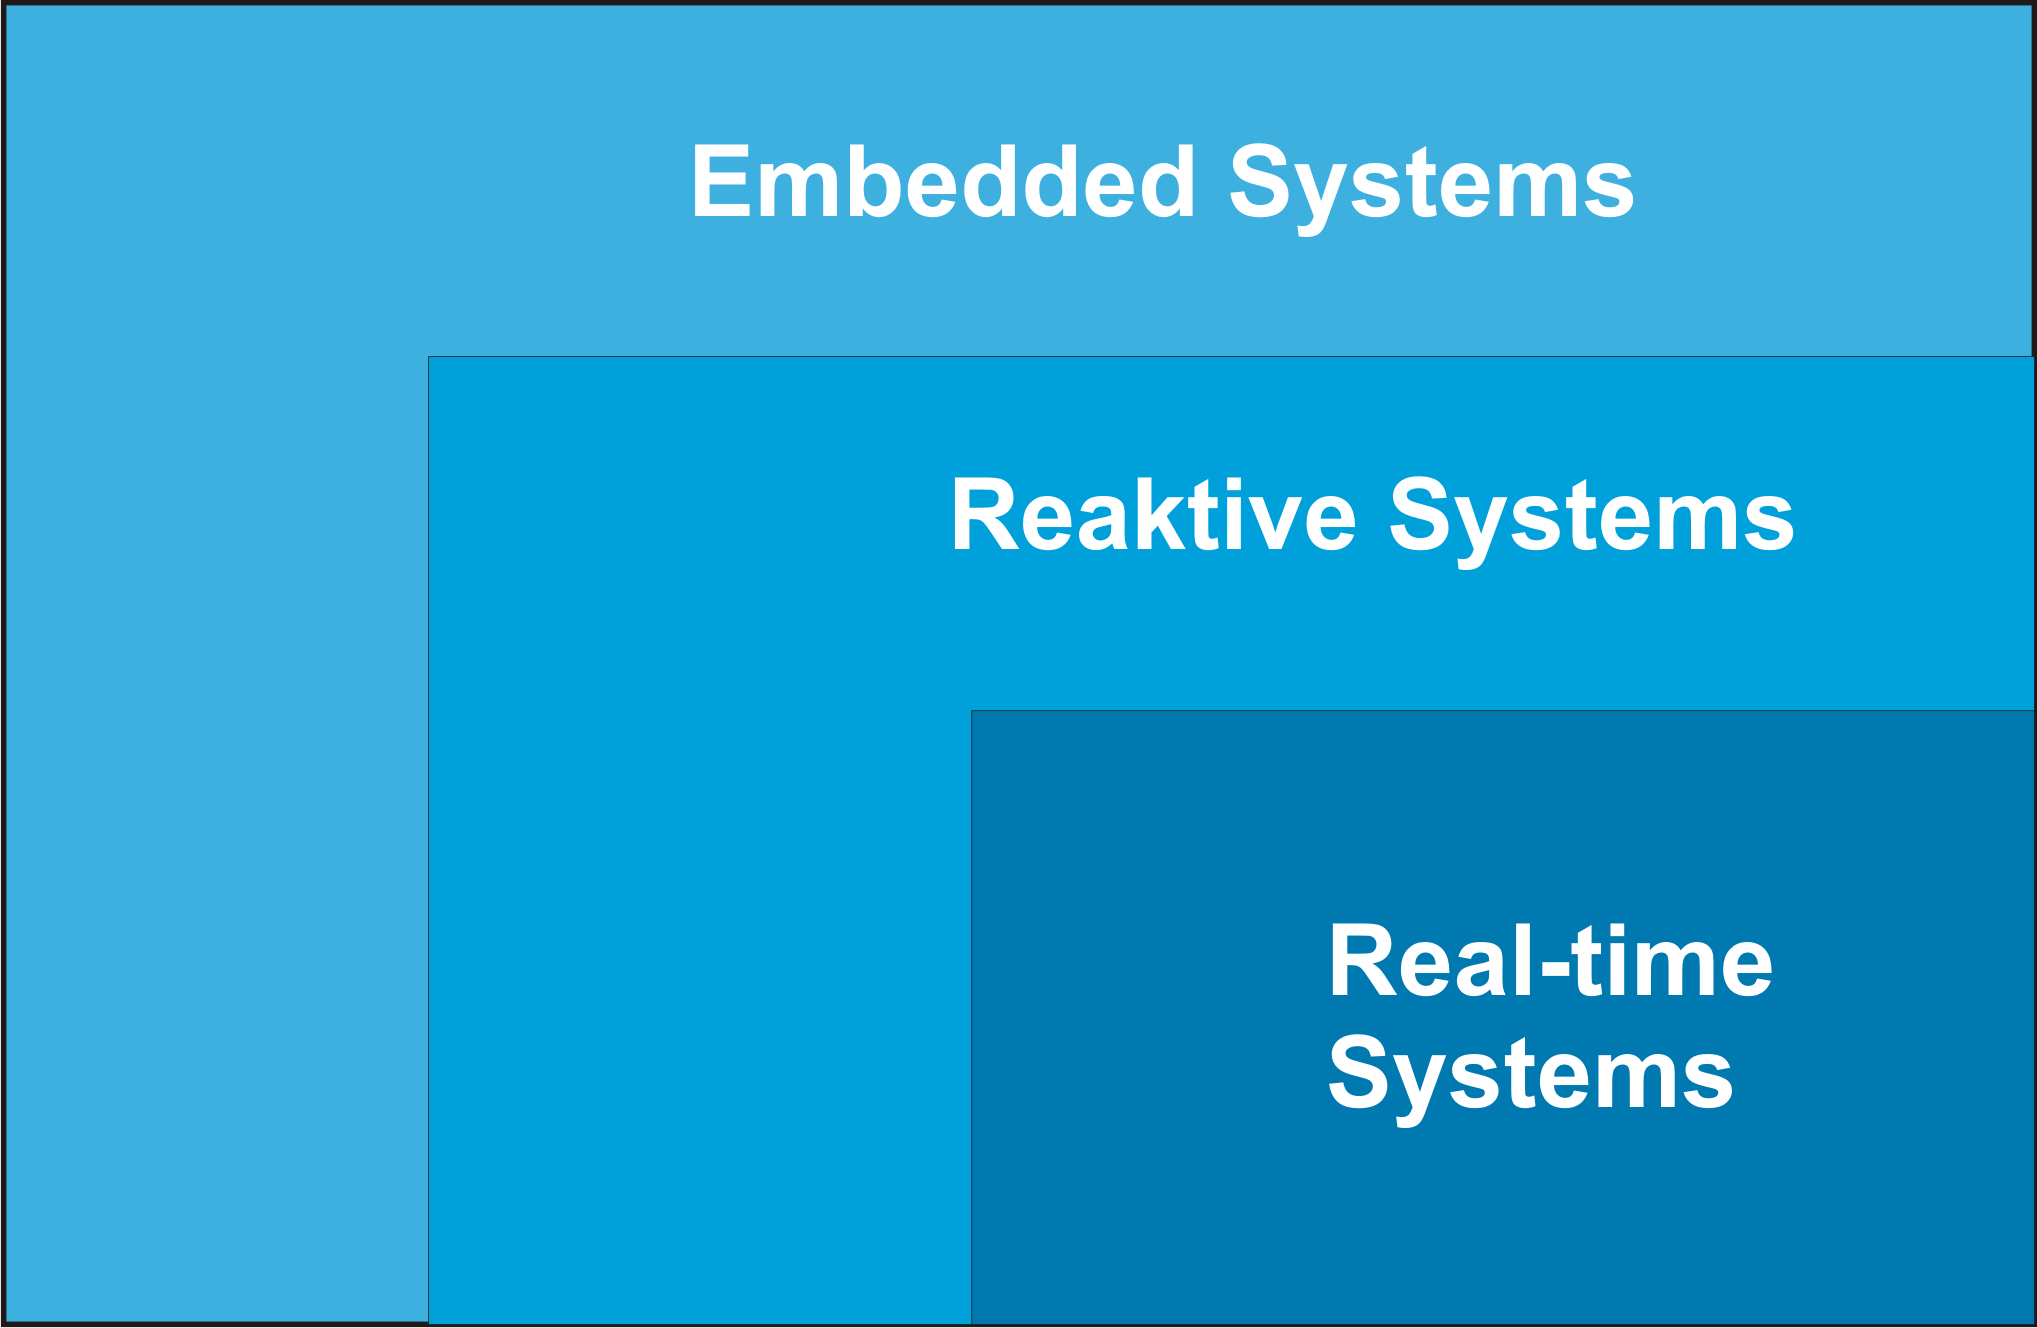
\epsfig{file=figures/Fig_2_1_Classification,width=0.7\textwidth}\\
	  \caption{Classification of embedded systems and real-time-systems}
     \end{center}
\end{figure}
\os{\newpage
}

\defn{def:embedded system}
{An \textbf{embedded system} is a special-purpose computer system designed to perform a dedicated function. Unlike a general-purpose computer, such as a personal computer, an embedded system performs one or a few pre-defined tasks, usually with very specific requirements, and often includes task-specific hardware and mechanical parts not usually found in a general-purpose computer. [Wikipedia]}


\defn{def:reaktive systems}
{``A \textbf{reactive system} is one which is in continual interaction
  with is environment and executes at a pace determined by
  that environment'' [Berg\'{e}, 1995]}

\bi
	\ite interaction with the system controlled by sensors or from the environment
	\ite specification of minimal and maximal response time
	\ite system could contain parallel and distributed parts (subsystems)
\ei

\defn{def:real-time systems}
{A \textbf{real-time system} have to give a responce as fast as required. So the system must respond to a signal, event or request fast enough to satisfy some requirement. Realtime often refers to process control and embedded systems}

\bi
	\ite a real-time operating system (RTOS) facilitates the creation of a real-time system
	\ite but real-time systems could operate without an RTOS
	\ite if a real-time system responds deterministically \pr hard real-time system
	\ite if a real-timesystem guarantees a deadline for responds \pr soft real-time system
\ei

\os{\newpage}
\begin{description}
\item[{\rot\bf Requirements }]~\\[-3ex]

\bi
	\ite concurrency \pr real-time systems are mostly concurrent
	\ite synchronization and communication \pr modeling the communication between distributed systems
	\ite portability and flexibility
	\ite programming elements \pr arithmetic operations, loops, and function calls should be available
	\ite non-standard I/O devices \pr switches, analogue and digital I/O
	\ite non-functional properties \pr e.g. fault-tolerance, disposability, EMC-properties, user friendliness, extendibility, expected life time, power consumption...
	\ite Co-Design aspects \pr modeling hard- and software functions
\ei
\item[{\rot\bf but }]~\\[-3ex]
\bi
	\ite models should be readable
	\ite models should have a hierarchical structure \pr ``humans not capable to understand systems
containing more than \begin{math} \sim \end{math} 5 objects''
\ei
\qbox{A model must be as simple as possible, but not simpler. [A. Einstein]}
\end{description}

\begin{figure}[!hbtp]
     \begin{center}
	  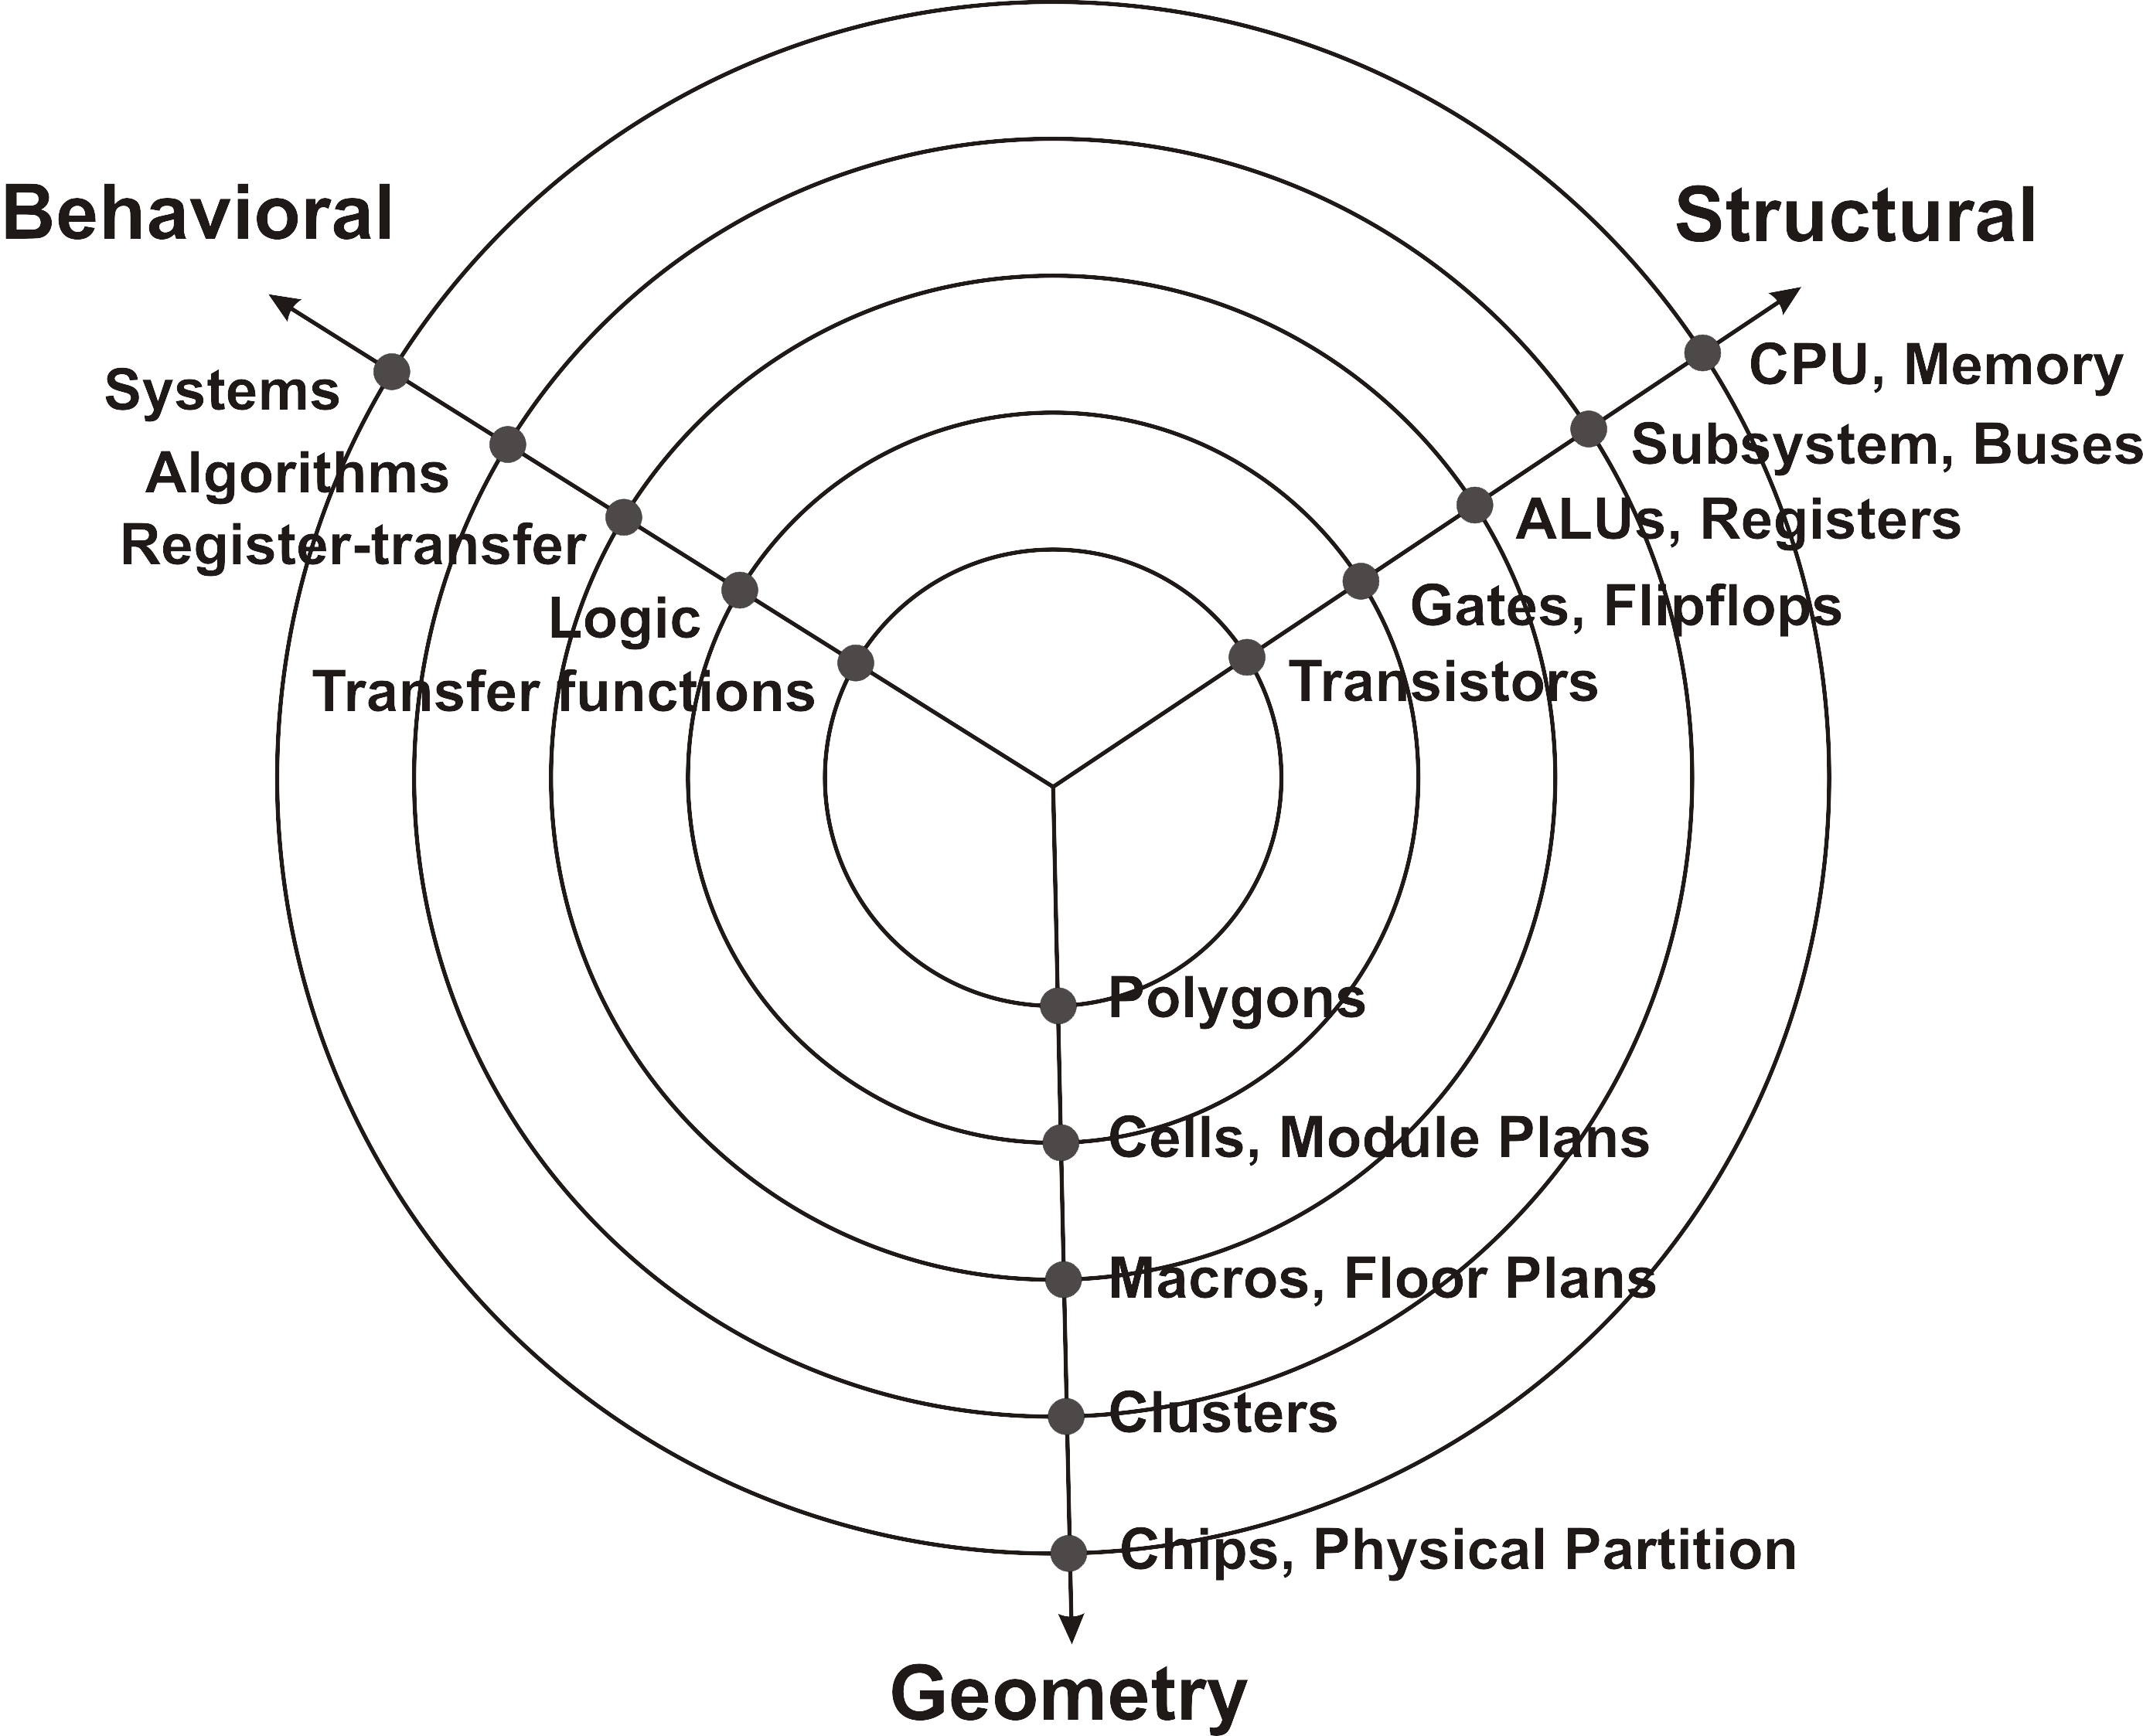
\epsfig{file=figures/Fig_2_2_Y_Chart_Gajski_Kuhn,width=0.8\textwidth}\\
	  \caption{Y-Chart from Gajski-Kuhn}
     \end{center}
\end{figure}
\os{\newpage}

\bi
	\ite a model could could change to different level in the Y-Chart
	\ite Y-Chart are focused on the hardware-design
	\ite concurrency and time behavior difficult to modeling
\ei

\begin{figure}[!hbtp]
     \begin{center}
	  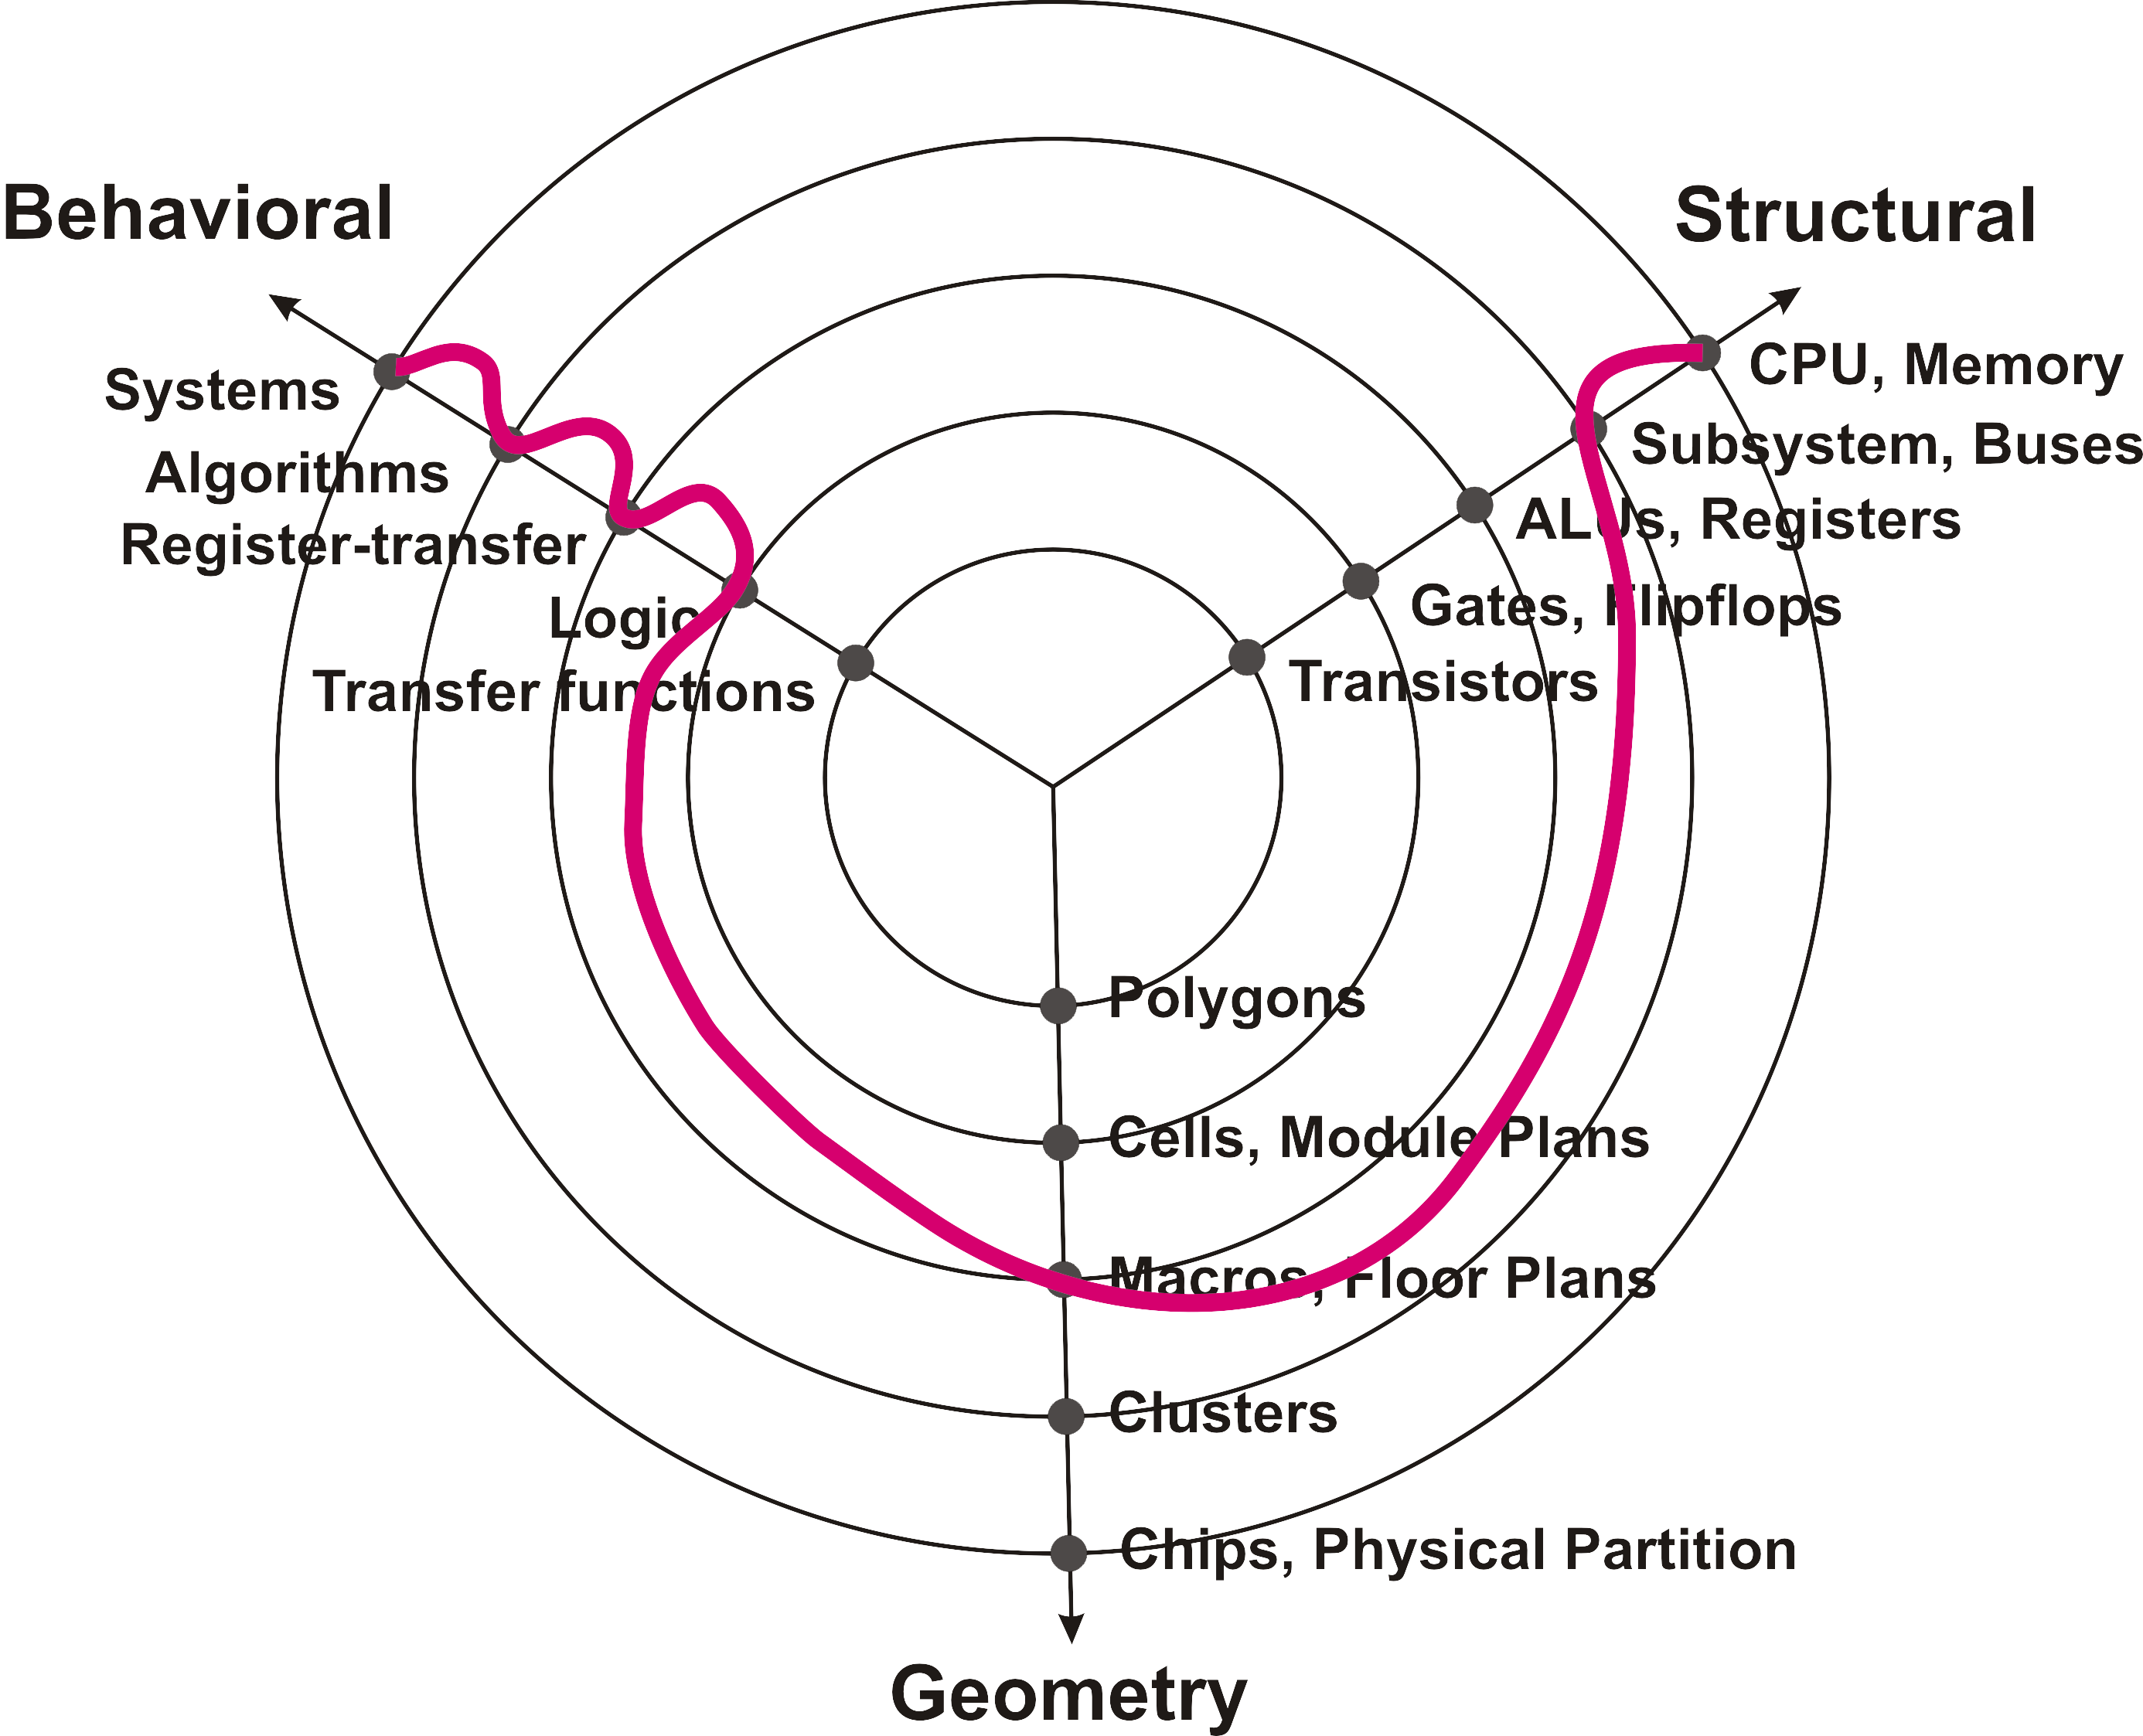
\epsfig{file=figures/Fig_2_3_Different_Level_Y_Chart,width=0.5\textwidth}\\
	  \caption{Different levels in a Y-Chart}
     \end{center}
\end{figure}
\os{\newpage}

\begin{figure}[!hbtp]
     \begin{center}
	  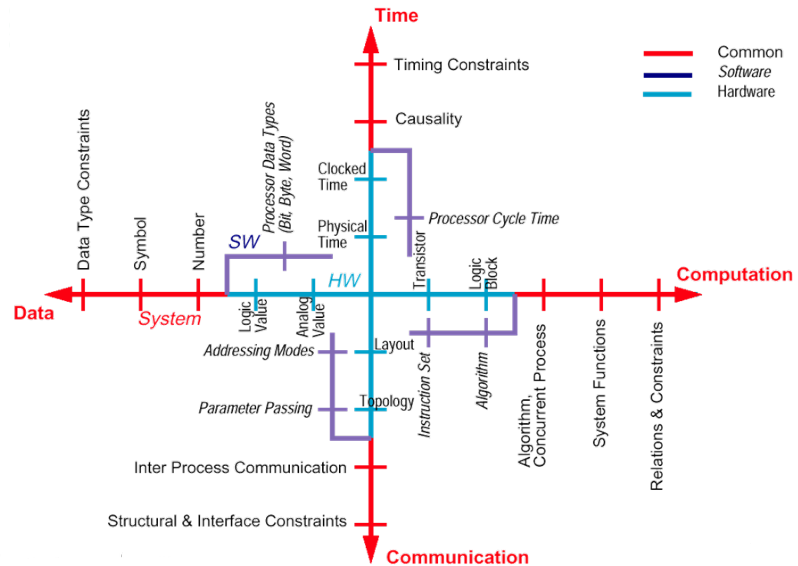
\epsfig{file=figures/Fig_2_4_4_D_CoDesign,width=0.9\textwidth}\\
	  \caption{Hardware and Software Co-Design}
     \end{center}
\end{figure}
\os{\newpage}

\begin{description}
\item[{\rot\bf Design methods }]~\\[-3ex]
\bigskip
\bi
	\ite capture and simulate
	\bi
		\ite specification of the embedded system (development)
		\ite generation of block diagrams (details not spezified)
		\ite simulation and verification
	\ei
\bigskip
	\ite describe and synthesize
	\bi
		\ite generate functions (software and hardware) from CAD-tools
		\ite logic synthesis as an integral component of the draft
		\ite use of hardware description languages (like VHDL)
	\ei
\bigskip
	\ite specify-explore-refine
	\bi
		\ite CAD/CASE-tools supports the explore-step (verification of different alternatives)
		\ite unfortunately these steps are not supported for all levels of the Co-Design
	\ei
\ei
\end{description}
\os{\newpage}
\begin{description}
\item[{\rot\bf Different views on a model }]~\\[-3ex]
\bigskip
\bi
	\ite  behavioral view
	\bi
		\ite use models or part of models as black boxes
		\ite focus on states, processes, procedures
	\ei
\bigskip
	\ite structural view
	\bi
		\ite specify the implementation of the system (e.g.connection of the components implies the behavior of the system)
		\ite processors, racks, printed circuit boards in the foreground
	\ei
\bigskip
	\ite view on physical components
	\bi
		\ite specify the physical characteristics of the components (e.g. expansion, layer, physical characteristics of the connections)
	\ei
\ei
\end{description}

\os{\newpage}
\begin{description}
\item[{\rot\bf Classification of models }]~\\[-3ex]
\bigskip
	\bi
		\ite a model which fulfils all the requirements of embedded system doesn't exit
		\ite actual models are focused on specific aspects
		\os{\bigskip}
		\bi
			\ite state space oriented
			\os{\bigskip}
			\ite activity oriented
			\os{\bigskip}
			\ite structural oriented
			\os{\bigskip}
			\ite data driven oriented
			\os{\bigskip}
			\ite heterogeneous oriented
		\ei
	\ei
\end{description}

%%%%%%%%%%%%%%%%%%%%%%%%%%%%%%%%%%%%%%%%%%%%%%%%%%%%%%%%%%%%%%%%%%%%%%%%%%%
\section{State Space Oriented Models}
%%%%%%%%%%%%%%%%%%%%%%%%%%%%%%%%%%%%%%%%%%%%%%%%%%%%%%%%%%%%%%%%%%%%%%%%%%%
\bigskip
\bi
	\ite Classical automata (FSM, \underline{f}inite \underline{s}tate \underline{m}achine) are state space models
	\ite Two different versions: Moore- and Mealy-Automata
\ei

\begin{figure}[!hbtp]
     \begin{center}
	  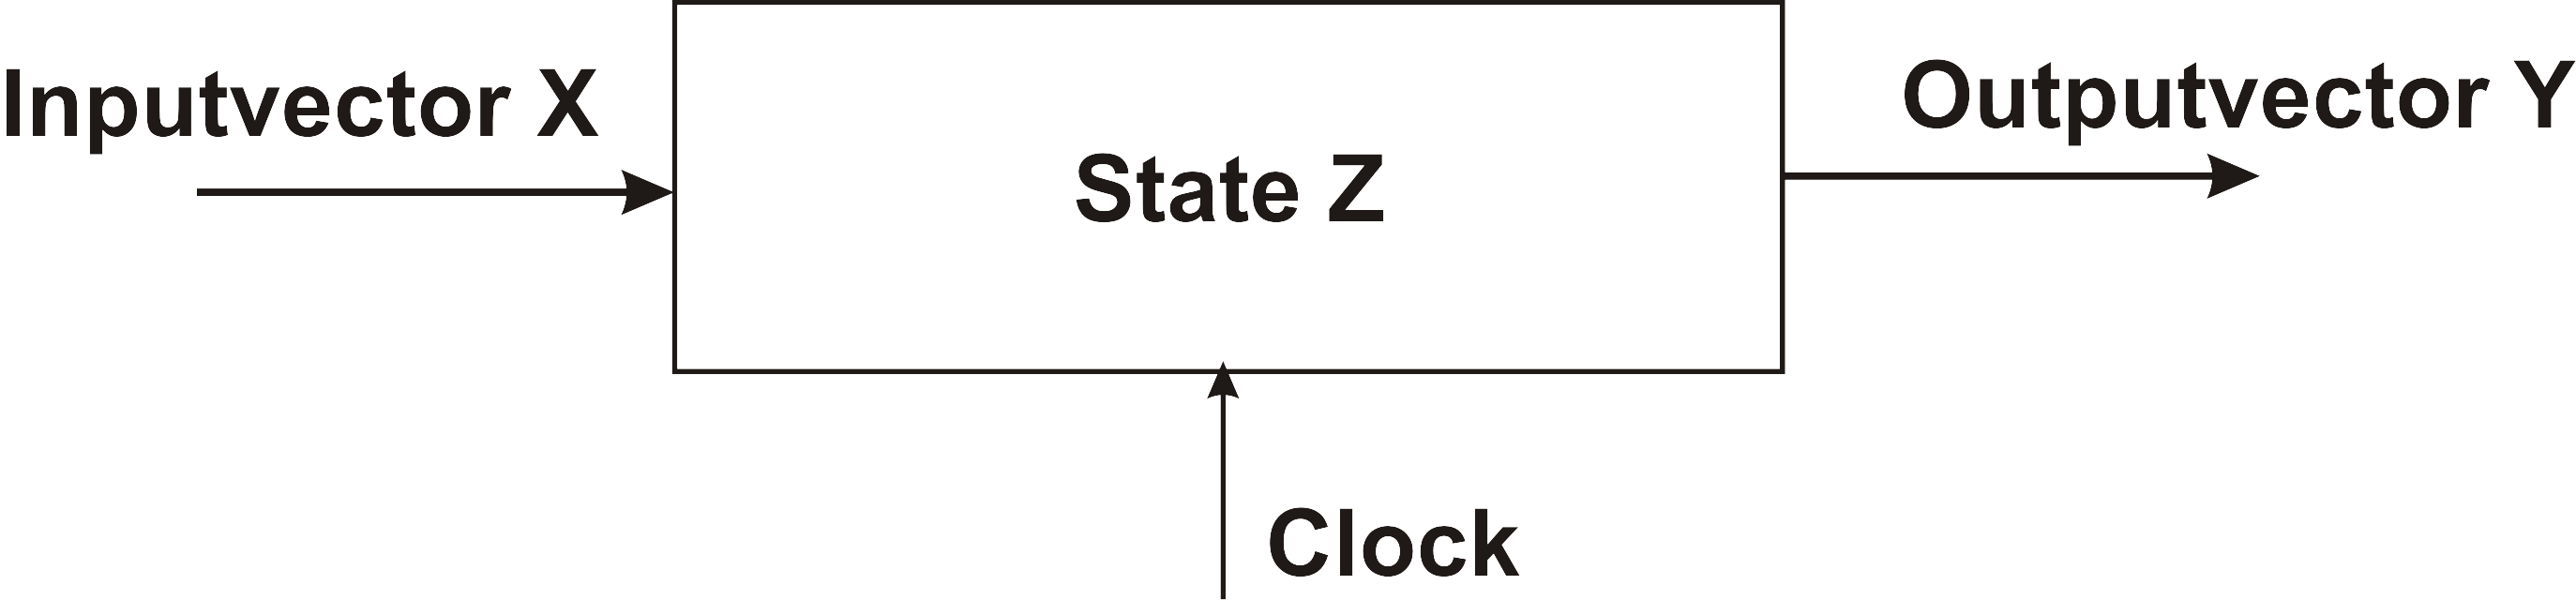
\epsfig{file=figures/Fig_2_5_FSM,width=0.9\textwidth}\\
	  \caption{Blockdiadram of a FSM}
     \end{center}
\end{figure}

\os{\newpage}

\begin{eqnarray*}
&Moore - automata\\
&Y = \lambda (Z); \ Z^{+} = \delta(X,Z)\\
\\
&Mealy - automata\\
&Y = \lambda(X,Z); \ Z^{+} = \delta(X,Z)\\
\\
&\lambda = output-function\\
&\delta = computes \ the \ next \ state \ Z^{+}
\end{eqnarray*}
\os{\newpage}

\begin{figure}[!hbtp]
     \begin{center}
	  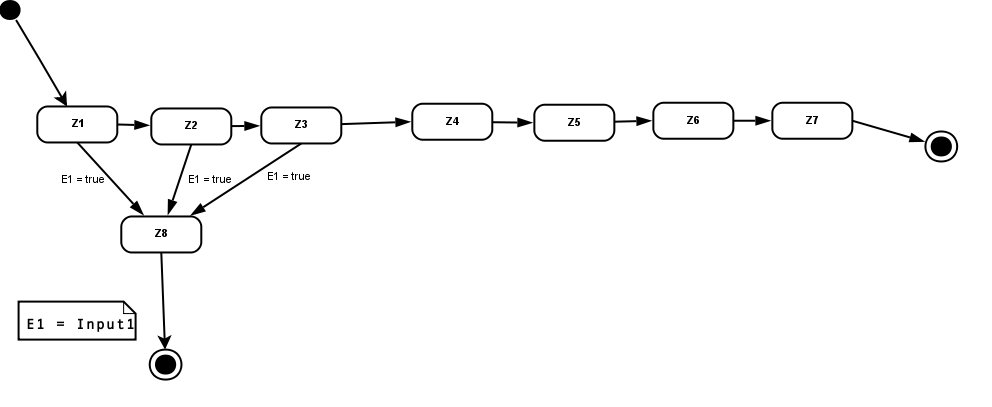
\epsfig{file=figures/Fig_2_6_FSM_Detail,width=0.8\textwidth}\\
	  \caption{FSM more in detail}
     \end{center}
\end{figure}

\os{\newpage}
\bi
	\ite FSM not useful for complex systems (to much details)
	\ite Introduction of hierarchy in the FSM \pr StateCharts [Harel, 1987]
\ei

\begin{figure}[!hbtp]
     \begin{center}
	  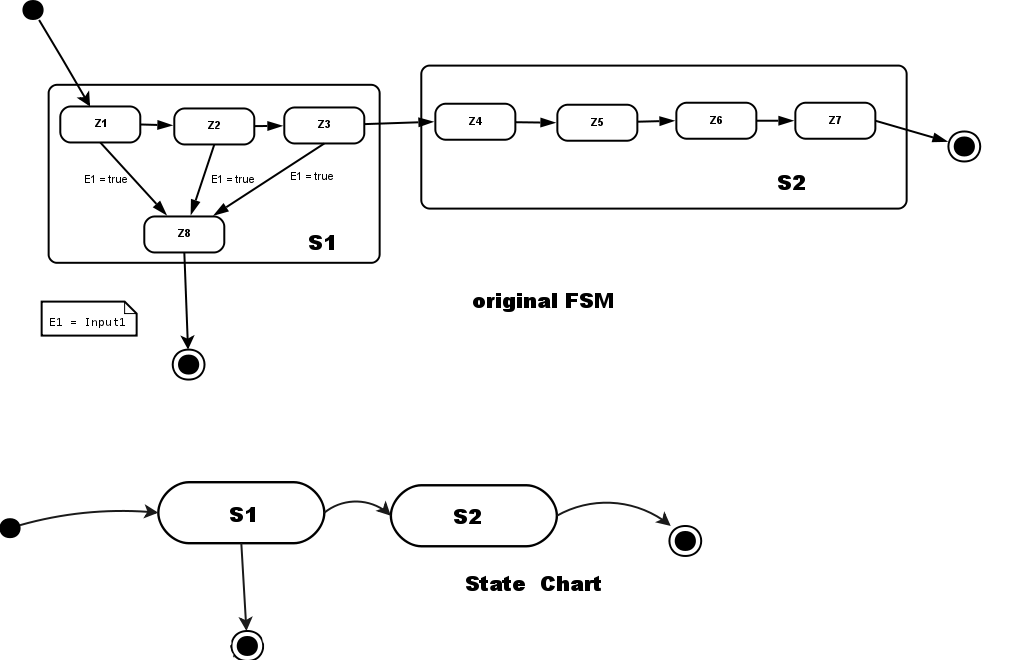
\epsfig{file=figures/Fig_2_7_State_Chart,width=0.7\textwidth}\\
	  \caption{State Chart}
     \end{center}
\end{figure}
\os{\newpage}

\defn{def:State Chart}
{Current states of FSMs are called \textbf{active states}.\\
States which are not composed of other states are called \textbf{basic
states}.\\
States containing other states are called \textbf{super-states}.\\
Super-states S are called \textbf{OR-super-states}, if exactly one of the
sub-states of S is active whenever S is active.}

\begin{figure}[!hbtp]
     \begin{center}
	  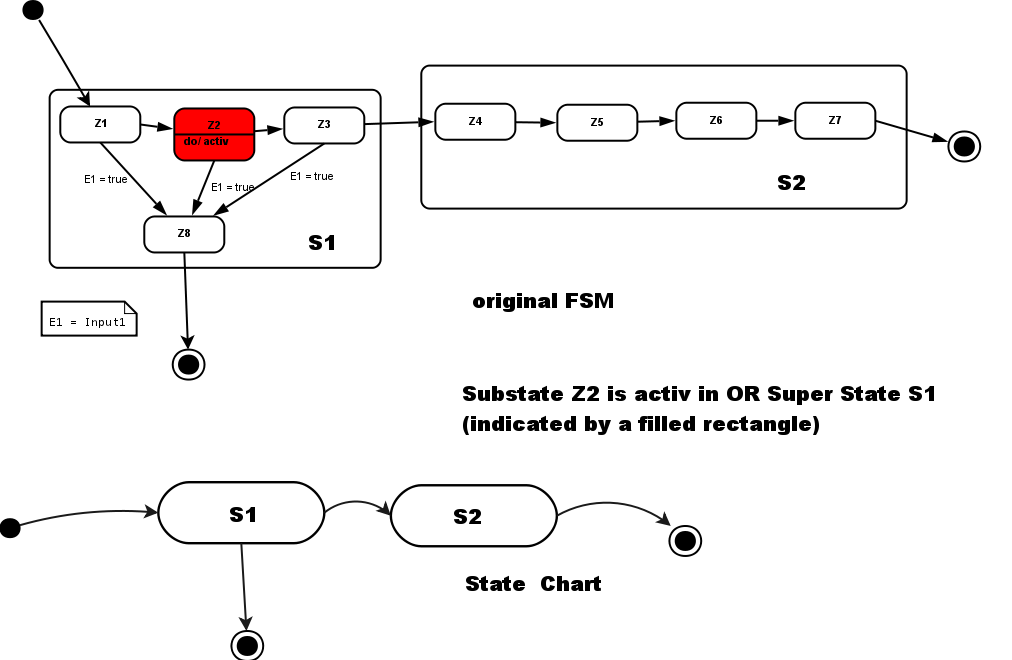
\epsfig{file=figures/Fig_2_8_Activ_Substate,width=0.6\textwidth}\\
	  \caption{Active Substate in a Super-State}
     \end{center}
\end{figure}

\os{\newpage}
\bi
	\ite In a OR-super-state only one sub-state is active
	\ite Modeling of concurrency not possible
\ei

\defn{def:AND-super-state}{A Super-states S are called \textbf{AND-super-states}, if in every AND-super-states exactly one sub-states is active.}


\begin{figure}[!hbtp]
     \begin{center}
	  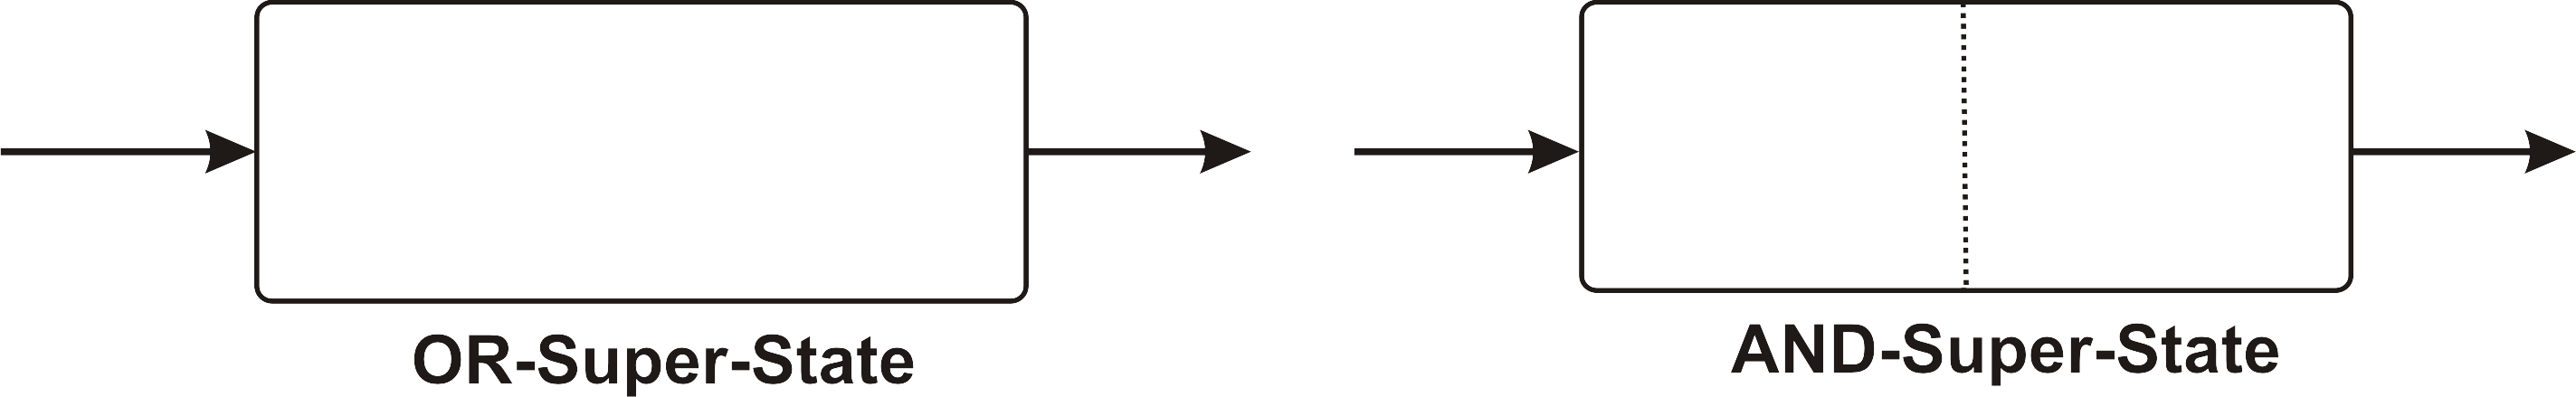
\epsfig{file=figures/Fig_2_9_OR_AND_Super_States,width=0.8\textwidth}\\
	  \caption{Concurrency in a AND-Super-State}
     \end{center}
\end{figure}
\os{\newpage}

\bi
	\ite In a AND-super-state \pr modeling of concurrent FSM possible
	\ite Implementation of a AND-super-state with a ``Product-FSM''
\ei

\begin{figure}[!hbtp]
     \begin{center}
	  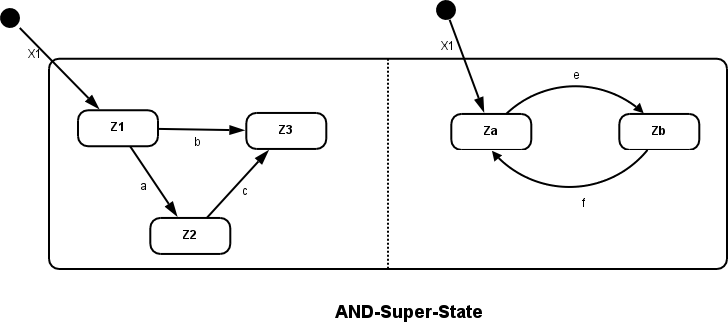
\epsfig{file=figures/Fig_2_10_AND_Superstate,width=0.8\textwidth}\\
	  \caption{Example of a AND-Super-State}
     \end{center}
\end{figure}

\os{\newpage}

\begin{figure}[!hbtp]
     \begin{center}
	  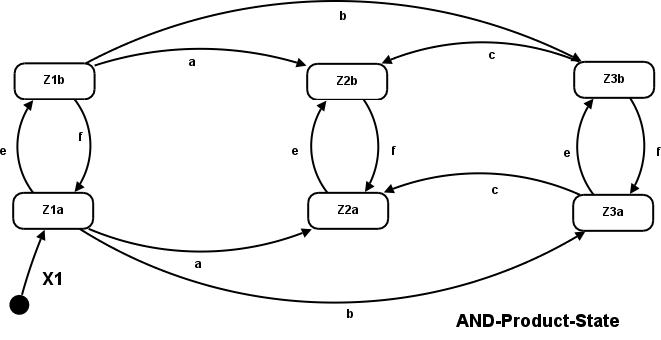
\epsfig{file=figures/Fig_2_10_AND_Product,width=0.9\textwidth}\\
	  \caption{Decomposition of a AND-Super-State}
     \end{center}
\end{figure}
\os{\newpage}

\bi
	\ite \textbf{Advantages of state charts modeling}
	\bi
		\ite hierarchy allows arbitrary nesting of AND- and OR-super
  states.
  		\ite semantics defined in a follow-up paper to original paper.
  		\ite large number of commercial simulation tools available (\textbf{StateMate, StateFlow, BetterState, ...})
		\ite some "back-ends" translate StateCharts into C or VHDL, thus enabling software or hardware implementations
	\ei
	\bigskip
	\ite \textbf{Disadvantages}
	\bi 	
		\ite generated C programs frequently inefficient
		\ite not useful for distributed applications
		\ite no program constructs
		\ite no description of non-functional behavior
		\ite no object-orientation
		\ite no description of structural hierarchy.
	\ei
\ei

\os{\newpage}
\bi
	\ite \textbf{Implementation of a Statemachine in C}
	\bi
		\ite As an example we take a coffee machine
        \ite State changes are caused by inputs (left/right/ready/!ready)
        \ite Output is not State Change -> Moore Machine		
	\ei
\ei
	\bigskip
	\begin{figure}[!hbtp]
     \begin{center}
	  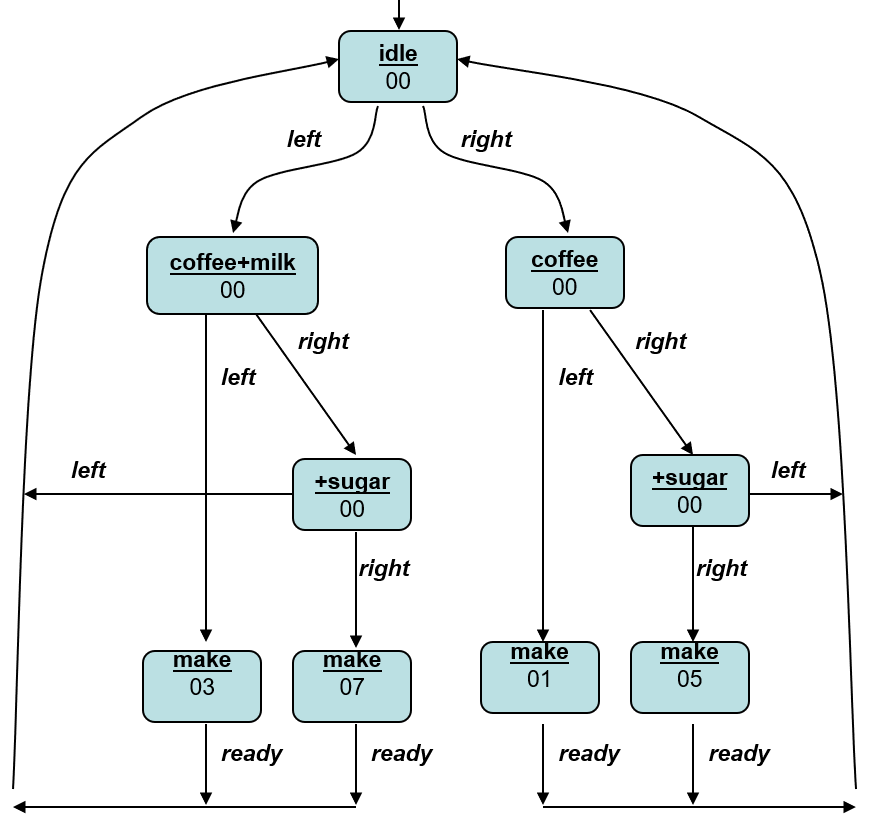
\epsfig{file=figures/Fig_2_10_CoffeeMachine_FSM,width=0.4\textwidth}\\
	  \caption{Coffee Machine FMS}
     \end{center}
\end{figure}

\os{\newpage}
\bi
	\ite \textbf{State Transition Table}
	
\ei
	\bigskip
	\begin{figure}[!hbtp]
     \begin{center}
	  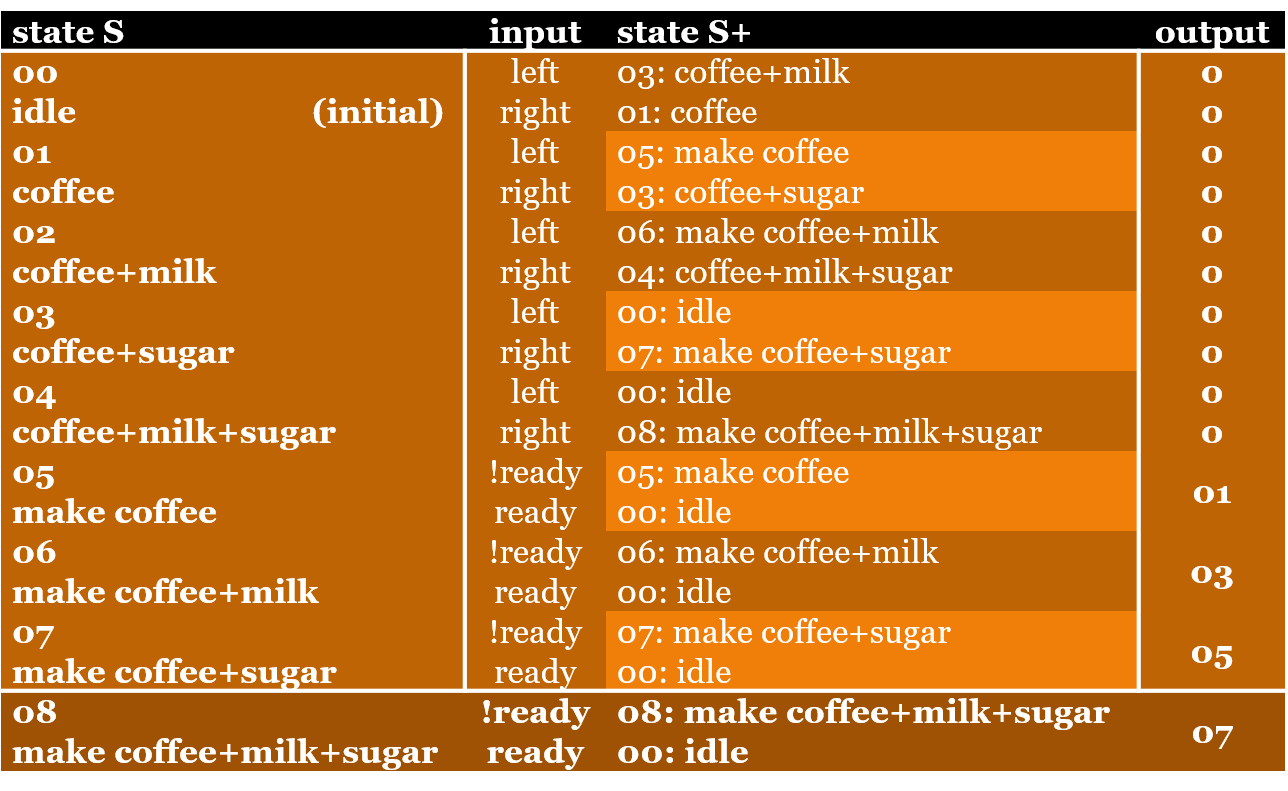
\epsfig{file=figures/Fig_2_10_CoffeeMachine_StateTable,width=0.7\textwidth}\\
	  \caption{Coffee Machine State Transition Table}
     \end{center}
\end{figure}

\os{\newpage}
\bi
	\ite \textbf{C Code - Definition of States}
	\bi
		\ite Always use ENUM to define states
        \ite Define an initial State	
	\ei
\ei
\begin{lstlisting}[language=C]
// --------------------------------------------------------
// the FSM states for the Coffee Automata
// --------------------------------------------------------
enum {  FSM_STATE_IDLE,  FSM_STATE_COFFEE, 		
        FSM_STATE_COFFEE_MILK,FSM_STATE_COFFEE_SUGAR,
        FSM_STATE_COFFEE_MILK_SUGAR,FSM_STATE_MAKE_COFFEE,
        FSM_STATE_MAKE_COFFEE_MILK, FSM_STATE_MAKE_COFFEE_SUGAR,
        FSM_STATE_MAKE_COFFEE_MILK_SUGAR,
};
// --------------------------------------------------------
int fsm_state = FSM_STATE_IDLE;
// --------------------------------------------------------
// --------------------------------------------------------
// the FSM outputs one for each state(Moore Automata model)
// --------------------------------------------------------
const int fsm_output[NUM_FSM_STATES] = {
        // output is fsm_output[fsm_state]
		0, 0, 0, 0, 0, 1, 3, 5 ,7								
        // bit0: add coffee, bit1: add milk, bit2: add sugar
 };
\end{lstlisting}

\os{\newpage}
\bi
	\ite \textbf{C Code - Inputs and Outputs}
	\bi
		\ite If possible use ENUM again	
	\ei
\ei
\begin{lstlisting}[language=C]
// --------------------------------------------------------
// the FSM outputs one for each state(Moore Automata model)
// --------------------------------------------------------
const int fsm_output[NUM_FSM_STATES] = {
        // output is fsm_output[fsm_state]
		0, 0, 0, 0, 0, 1, 3, 5 ,7								
        // bit0: add coffee, bit1: add milk, bit2: add sugar
 };
// ---------------------------------------------------------
// the FSM inputs
// ---------------------------------------------------------
enum {FSM_INP_NONE=0, FSM_INP_LEFT, FSM_INP_RIGHT, FSM_INP_READY };

\end{lstlisting}

\os{\newpage}
\bi
	\ite \textbf{C Code - State Transition}
	\bi
		\ite This function is called periodically
        \ite The period defines the response time of the system to input	
	\ei
\ei
\begin{lstlisting}[language=C]
int fsm_tic(int fsm_inp) // called periodically e.g. each 50 ms
{
	// the FSM transients realizing the state transient table
	// ------------------------------------------------------------
	switch (fsm_state) {
	case FSM_STATE_IDLE:
		if (fsm_inp == FSM_INP_LEFT) fsm_state = FSM_STATE_COFFEE;
		if (fsm_inp == FSM_INP_RIGHT) fsm_state = FSM_STATE_COFFEE_MILK;
		break;	
	case FSM_STATE_COFFEE:
		if (fsm_inp == FSM_INP_LEFT) fsm_state = FSM_STATE_MAKE_COFFEE;
		if (fsm_inp == FSM_INP_RIGHT) fsm_state = FSM_STATE_COFFEE_SUGAR;
		break;
	case FSM_STATE_COFFEE_MILK:
		if (fsm_inp == FSM_INP_LEFT) fsm_state = FSM_STATE_MAKE_COFFEE_MILK;
		if (fsm_inp == FSM_INP_RIGHT) fsm_state = FSM_STATE_COFFEE_MILK_SUGAR;
		break;
	case FSM_STATE_COFFEE_SUGAR:
		if (fsm_inp == FSM_INP_LEFT) fsm_state = FSM_STATE_IDLE;
		if (fsm_inp == FSM_INP_RIGHT) fsm_state = FSM_STATE_MAKE_COFFEE_SUGAR;
		break;
    case FSM_STATE_COFFEE_MILK_SUGAR:
		if (fsm_inp == FSM_INP_LEFT) fsm_state = FSM_STATE_IDLE;
		if (fsm_inp == FSM_INP_RIGHT) fsm_state = FSM_STATE_MAKE_COFFEE_MILK_SUGAR;
		break;
	case FSM_STATE_MAKE_COFFEE:   //here we wait for the coffeemaking to finish (ready!)
	case FSM_STATE_MAKE_COFFEE_MILK:
	case FSM_STATE_MAKE_COFFEE_SUGAR:
	case FSM_STATE_MAKE_COFFEE_MILK_SUGAR:
		if (fsm_inp == FSM_INP_READY) fsm_state = FSM_STATE_IDLE;
		break;
	default:
		;		// no state change
	}
	OUTPUT(fsm_output[fsm_state]);		// Moore FSM: one output per state
	return fsm_state;
}
\end{lstlisting}

\os{\newpage}
\bi
	\ite \textbf{Recipe for realizing a Moore Statemachine}
	\bi
		\ite Analyze the problem before coding plot a state diagram define the states
        \ite Use enums to encode states in a well readable form
        \ite Define outputs as enums with suitable encoding e.g. as bit-fields
        \ite Define input conditions causing the state transitions as enums as well
        \ite Realize a periodicaly called fsm-tic function realize transients and outputs
	\ei
\ei

\os{\newpage}
\bi
	\ite \textbf{Some Tools for creating and testing State Machines}
	\bi
		\ite The purpose of this list is not to give an exhaustive list of tools
        \ite The first part contains browserbased and free to use (at least with restrictions)
        \ite The second part contains free but installed tools
        \ite The final part commercial tools
        \ite
        \ite Browser based tools:
        \bi
            \ite Online Visual Paradigm - Commercial, with free option here:
            \ite https://online.visual-paradigm.com/app/diagrams/\#diagram:proj=0\&type=StateMachineDiagram
            \ite Nice editor
            \ite
            \ite Draw.Io - Free- Now located at
            \ite https://app.diagrams.net/
            \ite Many different options
            \ite
            \ite State Machine Simulator
            \ite http://ivanzuzak.info/noam/webapps/fsm\_simulator/
            \ite Powerful, complex editor and simulator/tester for FSM
        \ei
        \ite Free tools:
        \bi
            \ite Open Modelica available as part of the language and extensions in StateGraph
            \ite https://build.openmodelica.org/Documentation/Modelica.StateGraph.html
            \ite Powerful simulation, more complex, good integration for co-simulation
        \ei
        \ite Commercial tools:
        \bi
            \ite Matlab / Simulink Stateflow library
            \ite https://de.mathworks.com/products/stateflow.html
            \ite Powerful simulation, more complex, good integration into other libraries
        \ei
	\ei
\ei

%%%%%%%%%%%%%%%%%%%%%%%%%%%%%%%%%%%%%%%%%%%%%%%%%%%%%%%%%%%%%%%%%%%%%%%%%%%
\section{Activity Oriented Models}
%%%%%%%%%%%%%%%%%%%%%%%%%%%%%%%%%%%%%%%%%%%%%%%%%%%%%%%%%%%%%%%%%%%%%%%%%%%
\bigskip
\bi
	\ite modeling of the flow of datas in an embedded system \pr \textbf{DFG} (\underline{d}ata \underline{f}low \underline{g}raph)
	\ite node contains the activity
	\ite special nodes are input/output nodes and memory-nodes
	\ite shows the dependecies of data on all abstraction levels
	\ite ideally for the specification phase and as input for scheduling, because there don't exits sequential defaults
	\ite hierachical structure of DFG possible
\ei

\begin{figure}[!hbtp]
     \begin{center}
	  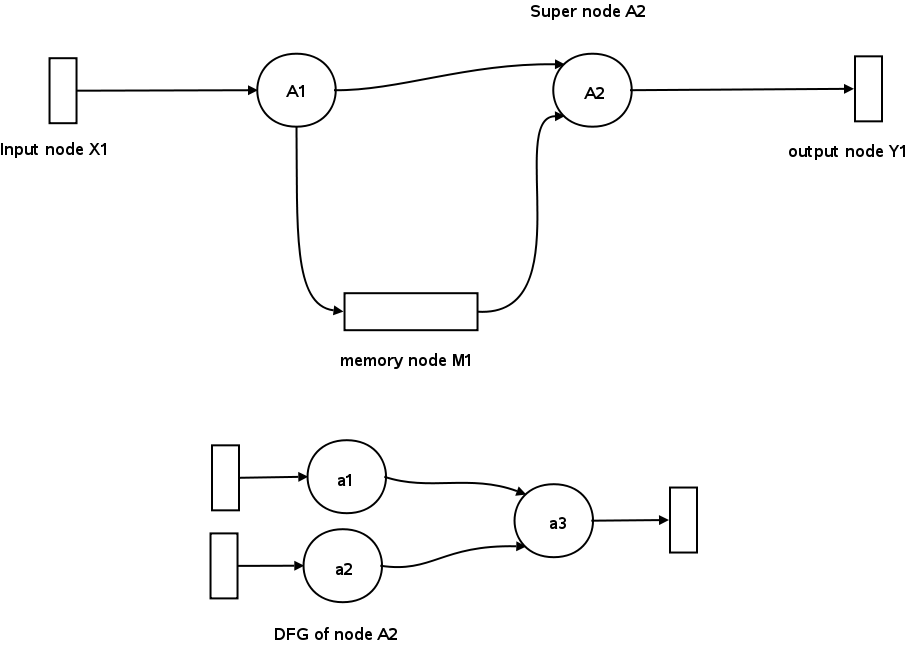
\epsfig{file=figures/Fig_2_11_DFG,width=0.9\textwidth}\\
	  \caption{Flow Graph}
     \end{center}
\end{figure}

\begin{figure}[!hbtp]
     \begin{center}
	  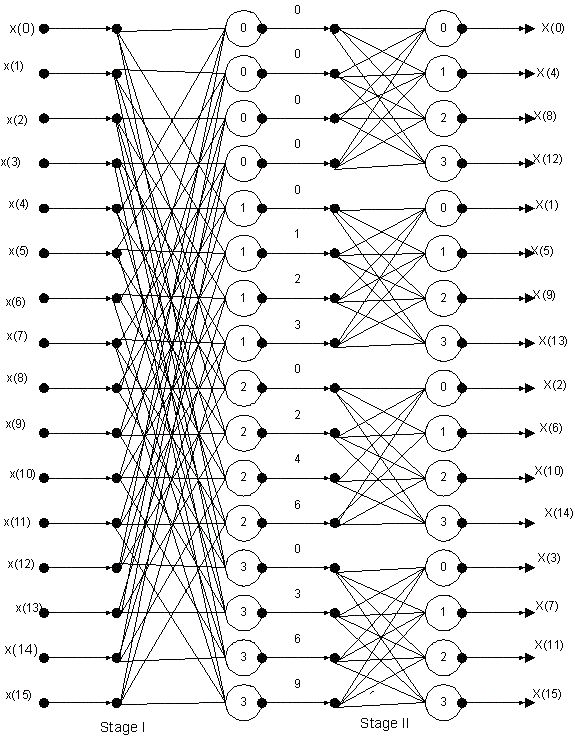
\epsfig{file=figures/Fig_2_12_DFG_FFT,width=0.5\textwidth}\\
	  \caption{DFG of a FFT-algorithm}
     \end{center}
\end{figure}

\os{\newpage}

\bi
	\ite extension of a DFG with control flow \pr \textbf{CFG}
	\ite introduction of ``control''-elements
	\ite edges transfers the control flow
	\ite CFG \pr Flow charts
\ei

\begin{figure}[!hbtp]
     \begin{center}
	  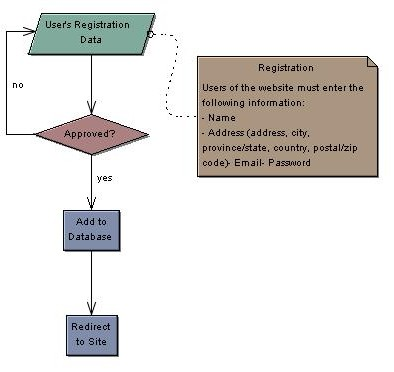
\epsfig{file=figures/Fig_2_13_FlowChart,width=0.7\textwidth}\\
	  \caption{Flow Chart of an Algorithm}
     \end{center}
\end{figure}
\os{\newpage}

\begin{description}
\item[{\rot\bf Message Sequence Charts (MSC) }]~\\[-3ex]
\bigskip
\bi
	\ite modeling of timing and scheduling behaviour
	\ite graphical means for representing schedules
	\bi
		\ite time is a separate axis (timing aspects are explicitly shown)
		\ite time axis vertical
		\ite activity axis horizontal
	\ei

\ei

\begin{figure}[!hbtp]
     \begin{center}
	  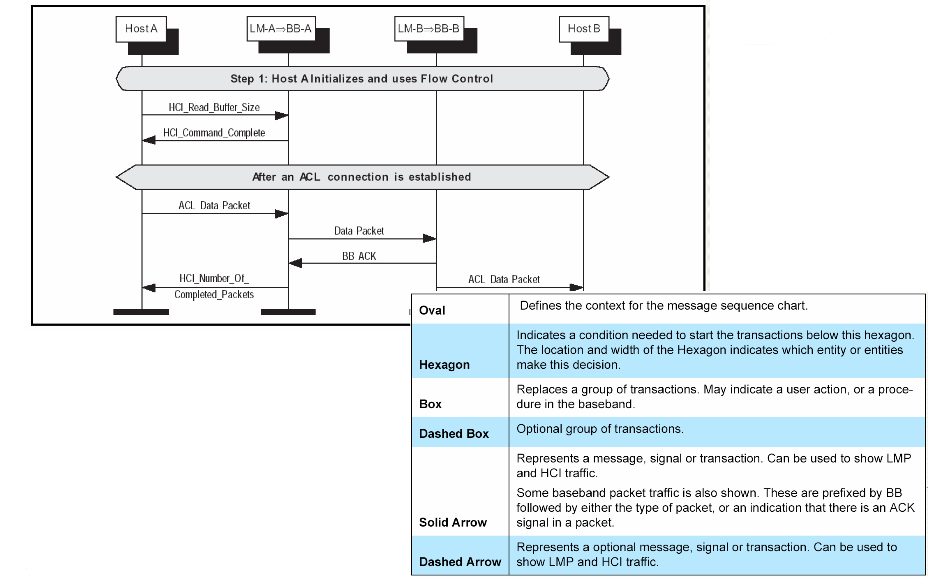
\epsfig{file=figures/Fig_2_14_MSG,width=1.0\textwidth}\\
	  \caption{Message Sequence Chart}
     \end{center}
\end{figure}

\os{\newpage}

\bi
	\ite \textbf{Advantages of activity oriented modeling}
	\bi
		\ite appropriate for visualizing schedules
		\ite proven method for representing schedules in transportation
		\ite hierarchy allowed in DFG and CFG  states.
  	\ei
	\bigskip
	\ite \textbf{Disadvantages}
	\bi
		\ite focused on one case, no timing tolerances or concurreny (MSC)
		\ite no description of non-functional behavior
		\ite no object-orientation
		\ite no description of structural hierarchy (MSC)
	\ei
\ei
\end{description}
